\section{Implementation and Deployment Configuration}
\label{sec:implementation}

In this section we present the details on how we implement~\videojam{}, \ie, the set of parameters of the architecture and the video analytics components. Further, we present our evaluation setup, including the evaluation metrics, the datasets we have select for evaluating the system, and the baselines we compare~\videojam{} with.

\subsection{Prototype Implementation}

We implement~\videojam{} with about 400 lines of Python 3 code, using the asyncio~\cite{asyncio} library to handle I/O operations of incoming frames and objects to process, and OpenCV v4.5.3 with \acrshort{cuda} v11.2.2 support for various vision models. With its simple design,~\videojam{} offers flexibility in incorporating any existing project, since only the communication component and the actual function (\eg, a Deep Neural Network model), are needed to be adapted to the existing one. The library is designed to easily support a variety of existing video analytics applications. We integrate the system in a docker image can be pulled from a public docker hub or built from the Dockerfile available in our public GitHub repository~\sidenote{The~\videojam{} implementation code is freely available at \href{https://github.com/ENSL-NS/VideoJam.git}{https://github.com/ENSL-NS/VideoJam.git}}. To evaluate the design effectiveness, we implement the functions of a typical traffic control application: vehicles' number plate detection.


\paragraph{Video Analytics Components.} We implement the vehicles' number plate detection pipeline by integrating the following video analytics functions: video source and decoder, background subtractor and vehicle detection (for fixed camera sources), YOLO object detection (for mobile sources), and number/license plate recognition.

\begin{figure}
	\centering
	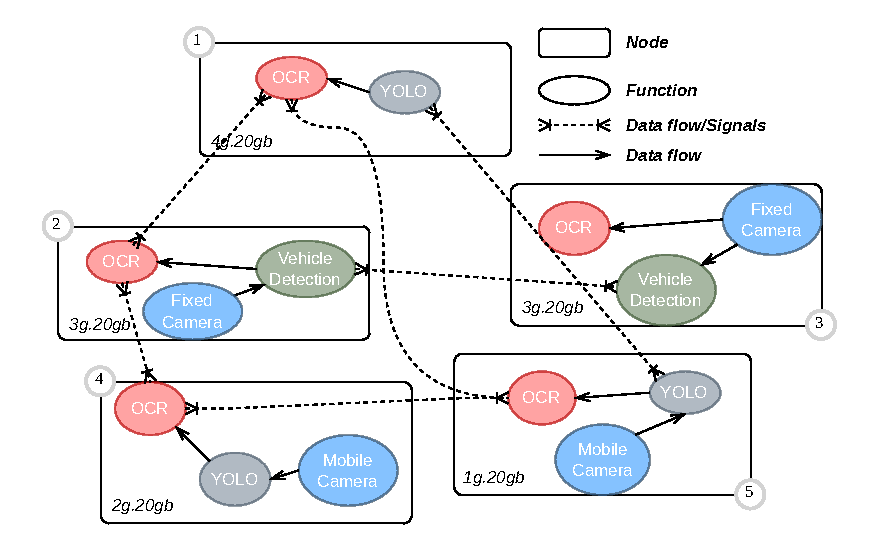
\includegraphics[width=\linewidth]{chapters/videojam/images/videojam_example_of_deployment.pdf}
	\caption{An example of heterogeneous deployment of~\videojam{}. Note that not all links between functions are represented to reduce image complexity.}
	\label{fig:example_deployment}
\end{figure}

The decoder represents the entry point of the pipeline and takes as input an encoded stream (for the evaluation in this paper we use pre-recorded videos, yet the system supports live streams as well). The decoded video frames are then passed on to the next function for further processing.

For fixed cameras, frames are transmitted to the background subtractor. The background subtractor is a function that generates a foreground mask using a static camera. This mask is then used on the current image to subtract the static scene, \ie, the background, while each moving scene is detected and classified as an object of interest. Extracted objects are then passed to the vehicle detection function, which embeds a machine learning model trained to detect vehicles within an image~\cite{vehicle_detection}. Detected vehicles are passed along to the next function, while other objects are discarded.

For detecting vehicles in mobile sources, we integrate a YOLOv5 model~\cite{jocher2020yolov5}. YOLOv5 is the fifth version of the YOLO (You Only Look Once) object detection model. It performs detection and classification, and returns a box for each object in the image taken in input, along with their classes with a high degree of accuracy. This is computationally intensive and is generally used on \acrshort{gpu}s to achieve fast and accurate results in real-time. There are many pre-trained check-points available, as well as input size pixel images. For our purposes, we use YOLOv5s with a high (640) and low (416) input pixels size. 

Finally, detected vehicles are passed to an object character recognition (OCR) function that used to detect license plates on cars. Numerous frameworks have been developed for this task. In our implementation we integrate Tesseract~\cite{ocr}, an open source OCR engine that combines traditional image processing techniques with modern machine learning methods to accurately recognize and convert text from images into a digital format.

We use these functions to create a heterogeneous application with two different pipelines. The first takes as input fixed video camera feeds passed along to the background subtractor, which forwards the data to the vehicle detector for classification before the final function, the license plate detection. The second pipeline takes data from a moving camera and processes them using YOLO, then passes the result to the license plate detection. This last function is shared by both pipelines for reuse and optimization. With such a deployment, a situation of workload imbalance can arise at any time, and forecasting becomes more challenging. The complete application used for deployment is presented in \Cref{fig:example_deployment}. All functions (except sources and background subtractor) of the same kind run load balancing and implement the~\videojam{} monitor and dispatcher. We have avoided drawing all the lines between the pairs (as specified in the caption) to avoid increasing the complexity of the figure.

\paragraph{System configuration and model tuning.} We configure the~\videojam{} load-balancing system using the parameters summarized in~\Cref{tab:configuration}. Regarding the predictive model, we opt for an architecture that minimizes inference time while guaranteeing acceptable performance. We choose a neural network (NN) with a single dense layer of 512 units trained over 100 epochs. The model takes in input a window of size $h$ and can predict a window of size $k$ (see~\Cref{tab:configuration} for the values of these parameters). We also tried out different architectures, such as a convolutional neural networks (CNN), and LSTMs. However, such models result to be difficult to use since (i) CNN requires a significant amount of time for the inference, although it has high levels of accuracy; (ii) in our case, LSTM presents poor performance in terms of both accuracy and inference time given its specific use on time series (different from our case).

\begin{table}
	\centering
	\begin{tabular}{p{1.5cm}p{6.5cm}}
    \toprule
	\textbf{Parameter} & \textbf{Value and description}                                                          \\
	\midrule
	\textbf{$\Delta$}  & 1 second (the monitoring duration)                                                      \\
	\textbf{$k$}       & 10, represents a monitoring window of $10*\Delta=10$ seconds                            \\
	\textbf{$h$}       & 50, the history for short-term forecasting                                              \\
	\textit{model}     & short-term forecasting: \acrshort{dnn} for Vehicle detection and Number plate OCR, none for YOLOv5 \\
	\bottomrule
	\end{tabular}
	\caption{\videojam{} configuration~\label{tab:configuration}}
\end{table}

\subsection{Evaluation Setup}\label{sec:setup}

\paragraph{Baselines.} We evaluate~\videojam{} compared against three different baselines: (i)~a video analytics pipeline that does not implement any load balancing, (ii)~one that implements Weighted Round Robin (WRR), and (iii)~Distream~\cite{zeng2020distream}, a state-of-the-art solution. In WRR, neighbors determine their processing rates based on an initial estimation, share this information with their neighbors, and collectively assign weights based on their capacity to create a load-balancing policy. They then apply this policy to distribute incoming workload to their local queues or to neighbors, with offloaded work being placed directly in a neighbor's local queue. For Distream, we start with the version available at the project repository\footnote{https://github.com/AIoT-MLSys-Lab/Distream/tree/main}. We then transform the Golang code into Python for integration into our deployment framework. Finally, we also adapt the code to support batch processing, mentioned in the article but not implemented in the open source version. The final code is also available on our public GitHub. Note that Distream does not support heterogeneous pipelines, thus we solely integrate the pipeline with YOLO into its architecture.

\paragraph{Deployment Infrastructure.} We conduct experiments deploying multiple docker containers on a server machine equipped with Nvidia A100 \acrshort{gpu}s (full specifications are shown in~\Cref{tab:grid5000}). For functions necessitating access to \acrshort{gpu} resources, we leverage the MIG (Multi-Instance \acrshort{gpu}) that Nvidia \acrshort{gpu} offers to split the available \acrshort{gpu}s into multiple instances. We emulate a heterogeneous edge infrastructure by splitting the \acrshort{gpu} into six nodes with heterogeneous compute cores (\ie, \textit{4g.20gb}, $2\times$~\textit{3g.20gb}, \textit{2g.10gb} and $2\times$~\textit{1g.5gb})~\cite{nvidiamig}. Given the lack of enough CPU cores we leave all containers to concurrently use all available CPUs. While this reduces the realism in terms of CPU isolation, the implemented functions mostly rely on the \acrshort{gpu} for heavier computations, thus not introducing unwanted bottlenecks to the setup. Finally, regarding network connectivity between containers, we emulate a realistic network configuration to the extent possible. For this reason, we not only limited the links between nodes to 1gbps, but also configured these links to have realistic latencies and bursts. For information, we used the following \textit{tc} command: \textit{rate 1gbit burst 16kbit latency 10ms}.

\begin{table}
	\centering
	\begin{tabular}{p{1cm}p{7cm}}
    \toprule
	\textbf{Model}  & Dell PowerEdge R7525                           			\\
	\textbf{CPU}    & AMD EPYC 7452 (Zen 2), 2 CPUs/node, 32 cores/CPU  	\\
	\textbf{Memory} & 128 GB																							\\
	\textbf{\acrshort{gpu}}    & 2 x Nvidia A100-PCIE-40GB, Compute capability: 8.0	\\
	\bottomrule
	\end{tabular}
	\caption{Server configuration used for experiments.}
	\label{tab:grid5000}
\end{table}

\paragraph{Evaluation metrics.} We evaluate the performance of~\videojam{} and the other baselines using three metrics: (i) the response time, (ii) the loss rate, and (iii) the total bandwidth utilization. The response time for a frame refers to the time elapsed from its introduction into the system (\ie, from the source)
to its complete processing by the last function in the pipeline. It can also be measured at the level of a specific pipeline function. For example, the response time for a frame measured at the vehicle detection level corresponds to the time elapsed between its entry into the pipeline and its exit from this function. A low response time is an indicator of the system's ability to quickly extract the
information generated by the application. The percentage of losses corresponds to the number of objects lost over the total number of objects to be processed.
In general, each function has a queue with a maximum number of items that can be held in it. When the incoming load exceeds a function's capacity, it begins to accumulate load in its queue. When the queue is full, any new incoming objects arrive they are dropped. Since we do not focus on function selection, losses
become the main indicator of accuracy reduction. Finally, total bandwidth utilization corresponds to the total amount of data transmitted during load balancing between functions. This is an important measure, as it enables us to measure the impact of the different approaches used on network resources.

\paragraph{Datasets.}
We use public real-world videos from YouTube for both fixed and mobile cameras. We selected a custom dataset of videos from YouTube for three reasons: (i) Existing mobile video datasets did not meet our requirements. For example, the BDD100k dataset~\footnote{http://bdd-data.berkeley.edu/}, widely used for analytics tasks, contains a good collection of traffic datasets from an on-board camera on cars in different weather conditions. However, the dataset contains only short sequences of videos lasting less than a minute or using under-sampled images. (ii) Using YouTube videos is a common standard in the state-of-the-art~\cite{zeng2020distream,zhang2022batch,lai2021top,wang2020surveiledge,elgamal2020sieve}. (iii) The selected dataset meets the diversity of requirements for the evaluation in this paper. The videos we selected include 11 videos from dashboard cameras mounted on cars traveling through various cities (\eg, Los Angeles~\footnote{https://www.youtube.com/watch?v=Cw0d-nqSNE8}), and nine fixed cameras mounted on street corners in the same cities~\footnote{https://www.youtube.com/watch?v=wqctLW0Hb\_0}. These recordings come in a variety of conditions, including normal to heavy traffic, as well as empty and crowded locations. As a result, the number of vehicles (\eg, cars, trucks) in the frames of these videos are variables, with minimum, maximum, mean, and median respectively of 0, 15, 3, and 3 per frame. Further, these videos are longer than the ones described in the previous dataset, and they span between 5 and 80 minutes (see~\Cref{tab:dataset}).

\begin{table}
	\centering
	\begin{tabular}{p{1.9cm}p{1.9cm}p{1.7cm}p{1.7cm}}
	\toprule
	\textbf{Type of camera} & \textbf{Duration (min)} & \textbf{Resolution} & \textbf{Total videos} \\
	\midrule
	Mobile        & 11-80                                                                                                     & 720p                & 9                      \\
	Fixed         & 5-60                                                                                                      & 720p                & 11                     \\
	\bottomrule
	\addlinespace        
	\end{tabular}
	\caption{Video cameras used for experiments.}
	\label{tab:dataset}
\end{table}